\RequirePackage{fix-cm}
\documentclass[11pt,a4paper]{article}
\usepackage{cmap}
\usepackage[T1]{fontenc}
\usepackage[sc]{mathpazo}
\linespread{1.04}
\DeclareFontShape{T1}{cmtt}{bx}{n}{<->ssub*cmtt/m/n}{}
\usepackage{colortbl}
\usepackage[margin=2.4cm]{geometry}
\usepackage{amsmath,amssymb,amsthm,mathtools}
\usepackage{booktabs,longtable,array,tabularx}
\usepackage{pdflscape}
\usepackage{enumitem}
\usepackage{xcolor}
\usepackage{tikz}
\usetikzlibrary{arrows.meta,positioning,calc,shapes.geometric,fit,backgrounds}
\usepackage{pgfplots}
\pgfplotsset{compat=1.16}
\usepackage[final]{microtype}
\usepackage[colorlinks=true,linkcolor=blue!50!black,citecolor=blue!50!black,urlcolor=blue!50!black]{hyperref}
\usepackage[capitalise]{cleveref}

\definecolor{accA}{HTML}{1F5E8C}
\definecolor{accB}{HTML}{8C4A1F}
\definecolor{accC}{HTML}{2E7D4F}
\definecolor{lvE}{HTML}{E8F1F8}
\definecolor{lvT}{HTML}{F1EEF8}
\definecolor{lvO}{HTML}{FBEFE6}

\newtheorem{theorem}{Theorem}
\newtheorem{corollary}{Corollary}
\theoremstyle{definition}
\newtheorem{definition}{Definition}
\newtheorem{example}{Example}
\theoremstyle{remark}
\newtheorem{remark}{Remark}

\newcommand{\Dstruct}{D_{\mathrm{struct}}}
\newcommand{\dstruct}{d_{\mathrm{struct}}}
\newcommand{\dspec}{d_{\mathrm{spec}}}
\newcommand{\AYM}{\mathcal{A}_{\mathrm{YM}}}
\newcommand{\SUNNS}{\mathcal{S}_{\mathrm{UNNS}}}
\newcommand{\HYM}{\mathcal{H}_{\mathrm{YM}}}
\newcommand{\Pset}{\mathcal{P}}
\newcommand{\sqs}{\sqrt{\sigma}}
\newcommand{\uns}{UNNS}
\setlist{itemsep=2pt,topsep=4pt}
\setlength{\parindent}{1.2em}
\setlength{\emergencystretch}{2em}
\renewcommand{\arraystretch}{1.12}

\title{\textbf{Structural Accessibility and Spectral Discreteness in Pure SU(3) Yang--Mills:}\\[2pt]
\large A \uns{} Reassessment of Vacuum Non-Crossability and the Mass Gap}
\author{UNNS Substrate Project}
\date{October 2026}

\begin{document}
\maketitle

\begin{abstract}
\noindent We investigate whether the Yang--Mills mass gap requires a structurally non-crossable neighborhood around the vacuum. An initial \uns{} non-crossability program distinguishes massive from gapless controls but fails to establish a universal refinement-stable vacuum boundary. We then test the alternative hypothesis that the Yang--Mills vacuum is structurally accessible within the same admissible domain. Across connected chromoelectric-field profiles, common-refinement analysis, canonical \uns{} structural chambers, an unsmoothed connected-correlator control, and a vacuum-subtracted continuum energy--momentum-tensor representation, no universal positive structural exclusion floor is detected. Independent continuum glueball spectroscopy nevertheless retains a strictly positive scalar excitation scale. The combined result supports the coexistence of structural vacuum accessibility with spectral discreteness and therefore separates structural proximity to the vacuum from spectral proximity to the vacuum.

\smallskip\noindent On the mathematical side, we prove a \emph{structural--spectral separation theorem}: a positive spectral gap does not by itself imply a structural exclusion neighborhood; it does so exactly when the excitation-energy functional is continuous at the vacuum in the structural topology, and a structural sequence approaching the vacuum under a persisting gap forces that continuity to fail. The theorem is elementary---it is essentially continuity---and we say so; its role is to locate the missing assumption of the original program. The substantive open problem is the specialization to Yang--Mills: constructing the structure-to-spectrum map $\Pi:\SUNNS\to\HYM$ and determining its topology. We do not prove $V\in\overline{\AYM}$, and nothing here addresses the Clay mass-gap problem.
\end{abstract}

\vspace{2pt}
\noindent\textbf{Keywords:} Yang--Mills mass gap; glueball spectrum; UNNS; structural accessibility; spectral gap; refinement; falsifiability.

\tableofcontents
\bigskip

%==============================================================
\section{Introduction: does a mass gap require a structural gap?}\label{sec:intro}

The Yang--Mills mass gap is a statement about the Hamiltonian spectrum: the lowest excited eigenvalue lies strictly above the vacuum energy, $E_1-E_0>0$. The \uns{} (Unbounded Nested Number Sequences) program studies recursion-generated structure, and one natural question within it is whether this spectral separation has a \emph{structural} shadow---whether the vacuum sits behind a wall in structure space that every non-vacuum admissible configuration must respect. This paper reports the outcome of testing that idea in two successive, fully frozen projects, and extracts from the outcome a precise mathematical statement about what such a wall would and would not follow from.

\subsection{Two distances from the vacuum}
Two different notions of ``distance from the vacuum'' are in play throughout.
\begin{itemize}
\item A \emph{structural} distance $\Dstruct(X,V)$, measured between an admissible structural representation $X$ of a gauge-invariant object (a field profile, a correlator ladder, an energy--momentum-tensor profile) and the vacuum representation $V$. It is a property of the \emph{configuration space of observables}.
\item A \emph{spectral} separation $\dspec(E_n,E_0)=E_n-E_0$, a property of the \emph{Hamiltonian eigenvalues}.
\end{itemize}
Nothing forces these to share a topology. The original hypothesis nevertheless implicitly identified them.

\subsection{The two competing hypotheses}
Let $\AYM$ be the admissible Yang--Mills-derived structural domain, $V$ the vacuum object, and $\Dstruct$ a structural distance. The first project tested
\begin{equation}\label{eq:Hiso}
\textbf{(H$_{\mathrm{iso}}$)}\qquad \Dstruct(X,V)\;\ge\;\delta>0\quad\text{for all admissible non-vacuum }X,\ \text{stable under refinement,}
\end{equation}
the \emph{non-crossability} (isolation) hypothesis. The second project tested the alternative
\begin{equation}\label{eq:Hacc}
\textbf{(H$_{\mathrm{acc}}$)}\qquad \exists\,X_n\in\AYM\setminus\{V\}:\ \Dstruct(X_n,V)\to0
\quad\text{while}\quad E_1-E_0>0 ,
\end{equation}
the \emph{accessibility} hypothesis: structural approach to the vacuum coexists with a nonzero spectral scale. The thesis of the paper is that the frozen evidence supports (H$_{\mathrm{acc}}$) within its stated architecture and does not support (H$_{\mathrm{iso}}$), and that this is mathematically unsurprising once the missing bridge condition is made explicit (\cref{sec:theorem}).

\subsection{Contributions, in three levels}
We keep three levels of statement strictly separate; the whole manuscript is organized around the separation.
\begin{center}
\renewcommand{\arraystretch}{1.25}
\begin{tabular}{@{}>{\columncolor{lvE}\raggedright\arraybackslash}p{2.9cm}>{\columncolor{lvT}\raggedright\arraybackslash}p{5.2cm}>{\columncolor{lvO}\raggedright\arraybackslash}p{6.5cm}@{}}
\textbf{Level 1: Empirical result} & \textbf{Level 2: Elementary theorem} & \textbf{Level 3: Open \uns{} theorem problem}\\
Structural accessibility and spectral positivity coexist in the tested pure-SU(3) representations (\cref{sec:stage2,sec:stage3,sec:bridge}). &
A spectral gap implies structural exclusion only under a continuity/coercivity bridge; accessibility plus a gap forces that bridge to fail (\cref{sec:theorem}). &
Construct the structure-to-Hilbert/spectral map $\Pi:\SUNNS\to\HYM$ and determine its topology (\cref{sec:implications}).
\end{tabular}
\end{center}

\begin{figure}[t]
\centering
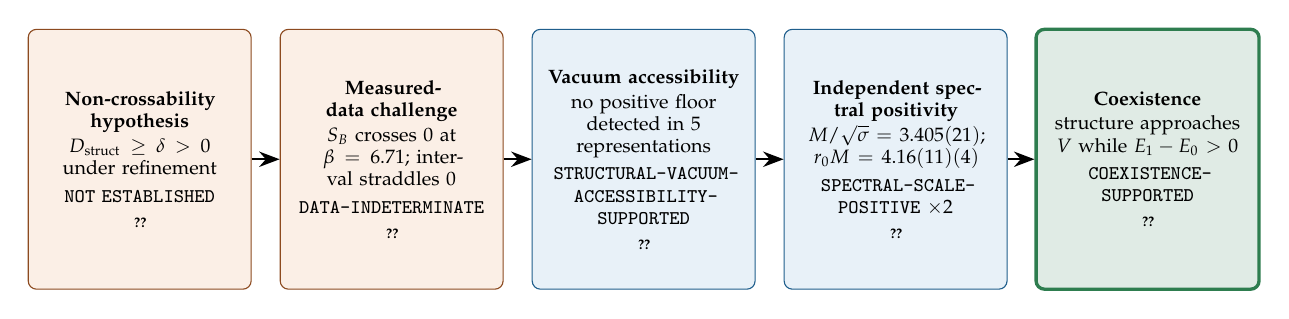
\begin{tikzpicture}[
 bx/.style={draw=accA,fill=lvE,rounded corners=3pt,text width=2.55cm,align=center,inner sep=4pt,font=\scriptsize,minimum height=3.3cm},
 hy/.style={draw=accB,fill=lvO,rounded corners=3pt,text width=2.55cm,align=center,inner sep=4pt,font=\scriptsize,minimum height=3.3cm},
 co/.style={draw=accC,fill=accC!15,rounded corners=3pt,line width=1.2pt,text width=2.55cm,align=center,inner sep=4pt,font=\scriptsize,minimum height=3.3cm},
 ar/.style={-{Stealth[length=2.6mm]},thick}]
\node[hy] (n1) at (0,0) {\textbf{Non-crossability hypothesis}\\[1pt]$\Dstruct\ge\delta>0$ under refinement\\[2pt]\texttt{NOT ESTABLISHED}\\[1pt]{\tiny \cref{sec:original}}};
\node[hy] (n2) at (3.2,0) {\textbf{Measured-data challenge}\\[1pt]$S_B$ crosses 0 at $\beta=6.71$; interval straddles 0\\[2pt]\texttt{DATA-\allowbreak{}INDETERMINATE}\\[1pt]{\tiny \cref{sec:original}}};
\node[bx] (n3) at (6.4,0) {\textbf{Vacuum accessibility}\\[1pt]no positive floor detected in 5 representations\\[2pt]\texttt{STRUCTURAL-\allowbreak{}VACUUM-\allowbreak{}ACCESSIBILITY-\allowbreak{}SUPPORTED}\\[1pt]{\tiny \cref{sec:stage2}}};
\node[bx] (n4) at (9.6,0) {\textbf{Independent spectral positivity}\\[1pt]$M/\sqrt\sigma=3.405(21)$;\\$r_0M=4.16(11)(4)$\\[2pt]\texttt{SPECTRAL-\allowbreak{}SCALE-\allowbreak{}POSITIVE} $\times2$\\[1pt]{\tiny \cref{sec:stage3}}};
\node[co] (n5) at (12.8,0) {\textbf{Coexistence}\\[1pt]structure approaches $V$ while $E_1-E_0>0$\\[2pt]\texttt{COEXISTENCE-\allowbreak{}SUPPORTED}\\[1pt]{\tiny \cref{sec:bridge}}};
\foreach \a/\b in {n1/n2,n2/n3,n3/n4,n4/n5} \draw[ar] (\a.east) -- (\b.west);
\end{tikzpicture}
\caption{Synthesis of the argument. Each box carries the frozen verdict of the corresponding stage; the arrows are logical, not causal. The final box is the output of the deterministic evaluator BRIDGE-III over frozen statuses and is not a theorem about Yang--Mills.}\label{fig:synth}
\end{figure}

\subsection{Roadmap and evidence grading}
\Cref{sec:original} presents the original non-crossability program fairly; \cref{sec:pivot} explains the conceptual pivot; \cref{sec:theorem} proves the separation theorem; \cref{sec:stage2,sec:stage3,sec:bridge} give the empirical body; \cref{sec:discussion,sec:implications} interpret it; \cref{sec:limits} states limitations and falsifiers; \cref{sec:conclusion} concludes. A single table (\cref{tab:verdicts}) lists every frozen verdict of both projects. Throughout, a verdict string is quoted exactly as frozen in the project records; results are graded as \emph{frozen empirical verdict}, \emph{limited empirical verdict}, \emph{structural interpretation}, or \emph{not established / not claimed}. Evidence classes follow the projects' own convention: Class~B means published measured data reconstructed from figures; Class~C means exact model controls anchored to a published fitted mass.

%==============================================================
\section{The original vacuum non-crossability hypothesis}\label{sec:original}

The first project, \texttt{UNNS\_YM\_GAP} (closed 2026-09-30 at stage YM-3B; terminal chamber CORR-I v0.1.2), began from the statement that \emph{gapless Yang--Mills continuation is structurally non-generable under refinement, whereas the massive branch is refinement-stable}; its stronger form was that the mass gap corresponds to a refinement-stable non-crossability boundary separating the vacuum from every non-vacuum admissible state. The intended physical bridge was $E(X)-E(V)\ge F_G(D_{\rm YM}(X,V))$ with $F_G(\delta_G)>0$; that bridge was never reached, and the project remained a structural investigation throughout. Four methodological requirements were frozen: gauge-invariant observables, actively constructed gapless adversaries, survival under common refinement, and a strict distinction between a structural diagnostic and a Hamiltonian theorem.

\subsection{YM-2A: vacuum-anchored spectral ladders}
The first representation used five glueball-state coordinates plus an explicit vacuum node, under four deformation families (\texttt{offset}, \texttt{upctrl}, \texttt{scale}, \texttt{gaponly}). STRUC-I did not reject the vacuum-compressed branch: the six-node ladder stayed structurally admissible even under a factor-1024 reduction of the vacuum gap. STRUC-PERC-I fragmented under some downward gap deformations, but the directionality test failed---upward displacement also fragmented, uniform scaling could preserve normalized connectivity, and gap-only deformation fragmented strongly. Connectivity collapse is therefore not equivalent to vacuum non-crossability, and the initial representation/test pair was falsified.

\subsection{YM-2B: the CORR-I diagnostic}
A short extracted mass ladder was judged too compressed to retain information about spectral support, so the project moved to Euclidean correlators $C(t)=\int_0^\infty\rho(E)e^{-Et}\,dE$ with $\rho\ge0$. CORR-I tests positivity, monotonicity, discrete log-convexity, effective-mass evolution, plateau behavior and Hankel/Hausdorff moment consistency, and measures compatibility with deliberately added low-energy spectral weight through the adversary
\begin{equation}
C_{\mathrm{adv}}(t)=(1-\alpha)\,C(t)+\alpha\,e^{-\mu(t-t_0)} .
\end{equation}
Rather than fix an arbitrary admixture, CORR-I computes the maximum compatible admixture $\alpha_{\max}(\mu)$ and reports the contraction ratio
\begin{equation}
R_{\mathrm{contract}}=\frac{\alpha_{\max}(\mu/m_{\mathrm{ref}}=10^{-3})}{\alpha_{\max}(\mu/m_{\mathrm{ref}}=1)} ,
\end{equation}
smaller values meaning stronger contraction of the near-zero compatibility envelope. This is a \uns{} diagnostic coordinate, not the physical gap. The stage coordinate used for refinement is the margin
\begin{equation}
S_B=\log_{10}\!\frac{R_{p=8}}{R_B}\qquad(\text{Class B;\ the Class C analogues are }S_{\rm fixed},S_{\rm match}),
\end{equation}
where $R_{p=8}$ is the contraction ratio of the hardest member of the positive-spectral Gamma family of gapless adversaries and $R_B$ that of the measured (or massive-control) correlator. $S>0$ means the massive-side signature lies on the contracted side of the hardest adversary; $S\le0$ means the proposed boundary has been reached or crossed.

At the finest AT20 resolution the massive control gave $R_{\rm massive}\approx0.007688$ against gapless Gamma members $R=0.5009,\,0.3269,\,0.1786,\,0.0845,\,0.0377$ for $p=0.5,1,2,4,8$ (factors $65.2,\,42.5,\,23.2,\,11.0,\,4.90$ above the massive control); every gapless member remained positive-spectral consistent. Positive spectral consistency alone therefore did not force the massive-side response. The stage closed provisionally with \texttt{VACUUM-\allowbreak{}BOUNDARY DIAGNOSTIC ESTABLISHED; REFINEMENT TEST REQUIRED}. The idea thus had genuine empirical motivation: CORR-I did separate massive from gapless adversaries.

\subsection{YM-3A: model-refinement persistence (Class C)}
Using exact mass-anchored exponential controls over the eight-level Athenodorou--Teper refinement sequence \cite{AT20}, the frozen result was \texttt{MODEL-\allowbreak{}REFINEMENT PERSISTENT}: at all eight levels the massive control stayed on the massive side of the fixed hardest gapless reference and of every $\beta$-matched Gamma control, with the full ordering $R_{0.5}>R_1>R_2>R_4>R_8>R_{\rm massive}$ retained. The matched margin grew from $S_{\rm match}=0.8067$ at $\beta=5.6924$ to $1.5892$ at $\beta=6.50$ (\cref{tab:ym3a}, \cref{app:data}). This is a genuine positive result, but only for the model family: an exponential built from a published fitted mass carries no measured effective-mass fluctuation, contamination or covariance, so YM-3A establishes model-refinement persistence and not refinement persistence of measured correlators.

\subsection{YM-3B: the measured-data challenge (Class B)}
The decisive test used four ordered pure-SU(3) ensembles of Sakai and Sasaki \cite{SS23} at $\beta=6.20,\,6.40,\,6.71,\,6.93$, reconstructing normalized variational-eigenvalue proxies from the published $A_1^{++}$ effective-mass trajectories on a common physical-time grid. The central margins were
\begin{equation}
S_B=\{+0.020350,\ +0.035867,\ -0.003395,\ +0.051851\},
\end{equation}
so the central trajectory \emph{crossed} the proposed boundary at $\beta=6.71$, where the matched ordering failed because $R_B>R_{p=8}$ (\cref{tab:ym3b}). The negative sign survived PCHIP interpolation ($-0.003948$) and all three nested ladder lengths ($S_B^{L5}=-0.007663$, $S_B^{L6}=-0.006666$, $S_B^{L7}=-0.003395$). However, the preregistered 2000-draw pointwise-no-covariance uncertainty ensemble at $\beta=6.71$ gave a 95\% interval $[-0.027454,\,+0.019320]$ with median $-0.003285$ and a negative fraction $0.6065$, straddling zero; the other three $\beta$ values were sign-stable (\cref{fig:SB}). The frozen verdict is therefore \texttt{DATA-\allowbreak{}INDETERMINATE}: the crossing is not erased, but available published-figure precision cannot classify it as a stable falsification.

\subsection{Closure}
The central hypothesis was recorded as \texttt{NOT ESTABLISHED}; YM-4 (a bridge theorem under the original premise) was not entered and further tests (Liang14 replication, Chen06 extension, additional source search, CORR-I redesign) were cancelled. We stress what the record does \emph{not} say: it does not call the picture refuted, does not claim that no structural boundary exists, and neither proves nor disproves the physical mass gap. It does, however, expose a consequence that motivates the second project: across the tested representations the vacuum could not be maintained as an object external to admissible structure behind a universal wall.

\begin{figure}[t]
\centering
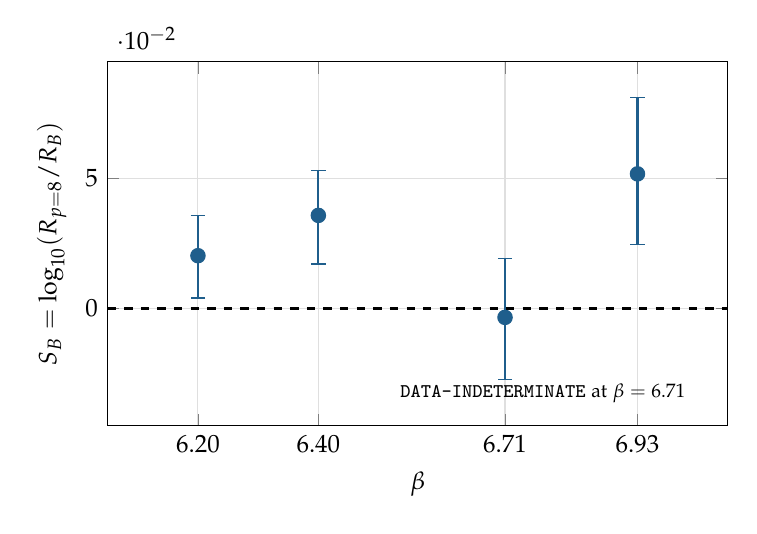
\begin{tikzpicture}
\begin{axis}[width=0.78\textwidth,height=6.2cm,xlabel={$\beta$},ylabel={$S_B=\log_{10}(R_{p=8}/R_B)$},xmin=6.05,xmax=7.08,ymin=-0.045,ymax=0.095,xtick={6.2,6.4,6.71,6.93},xticklabels={6.20,6.40,6.71,6.93},grid=major,grid style={gray!25},tick label style={font=\small},label style={font=\small}]
\addplot[dashed,thick,black] coordinates {(6.05,0)(7.08,0)};
\addplot[only marks,mark=*,mark size=2.6pt,accA,error bars/.cd,y dir=both,y explicit,error bar style={thick}] table[row sep=\\,x index=0,y index=1,y error plus index=2,y error minus index=3] {
6.2 0.020350 0.015308 0.016297\\
6.4 0.035867 0.017227 0.018700\\
6.71 -0.003395 0.022715 0.024059\\
6.93 0.051851 0.029343 0.027126\\
};
\node[font=\scriptsize,anchor=south west] at (axis cs:6.52,-0.040) {\texttt{DATA-\allowbreak{}INDETERMINATE} at $\beta=6.71$};
\end{axis}
\end{tikzpicture}
\caption{Class B margin $S_B=\log_{10}(R_{p=8}/R_B)$ at the four Sakai--Sasaki ensembles \cite{SS23}. Dots: central values; bars: preregistered 2000-draw 95\% intervals (central 2.5\%--97.5\% quantiles); the dashed line is the proposed boundary $S_B=0$. Only $\beta=6.71$ is sign-unstable, and there the interval straddles zero (\texttt{DATA-\allowbreak{}INDETERMINATE}).}\label{fig:SB}
\end{figure}

%==============================================================
\section{From non-crossability to structural accessibility}\label{sec:pivot}

The pivot is conceptual. A mass gap separates \emph{eigenvalues}; a structural neighborhood describes \emph{configurations or observables}. These live in different spaces with no a priori common topology, so a spectral gap need not induce a structural wall. The second project, \texttt{UNNS\_VACUUM\_CONTINUITY}, froze the corresponding ontology in its Stage~1: the vacuum is treated as an \emph{internal closure object} of the admissible domain,
\begin{equation}
V\in\overline{\AYM\setminus\{V\}},\qquad\text{primary hypothesis}\quad \inf_{X\in\AYM\setminus\{V\}}\Dstruct(X,V)=0,
\end{equation}
with the isolation alternative $\exists\,\delta_V>0$ such that $\Dstruct(X,V)\ge\delta_V$ for every sufficiently refined admissible non-vacuum structure in the tested representation class. Stage~1 deliberately did \emph{not} adopt the stronger language ``basin'', ``attractor'' or ``fixed point''. Its physical shorthand, frozen as an interpretive (not theorem-level) statement, is that the mass gap separates eigenvalues, not necessarily structural neighborhoods.

The primary independent structural representation is VREF-I, a vacuum-referenced profile representation: an ordered spatial profile of a gauge-invariant observable (connected action/energy density or an equivalent) referenced to an independently defined vacuum baseline. Refinement is common-support refinement across independent lattice resolutions. A structural-vacuum conclusion was not allowed to rest on a single negative diagnostic value; it required common refinement, vacuum-directed physical profiles, zero-floor versus positive-floor model competition, uncertainty control, independent chambers, smoothing and interpolation sensitivity, an operator change, and geometry sensitivity, with negative and indeterminate results preserved without retuning.

\Cref{sec:theorem} formalizes why this pivot is not ad hoc: it identifies exactly which assumption separates (H$_{\rm iso}$) from (H$_{\rm acc}$).

%==============================================================
\section{A structural--spectral separation theorem}\label{sec:theorem}

\subsection{Setting}
\begin{definition}[Structural--spectral data]
A \emph{structural--spectral system} consists of a metric space $(\mathcal S,d)$ of structural states; a distinguished vacuum $V\in\mathcal S$; a set $\Pset\subseteq\mathcal S\setminus\{V\}$ of \emph{physical non-vacuum excitations}; and an \emph{excitation-energy functional} $\varepsilon:\mathcal S\to[0,\infty)$ with $\varepsilon(V)=0$. The system is \emph{gapped} with gap $\Delta>0$ if
\begin{equation}\label{eq:gap}
\varepsilon(X)\ge\Delta\qquad\text{for all }X\in\Pset .
\end{equation}
It has a \emph{structural exclusion radius} $\delta>0$ if $d(X,V)\ge\delta$ for all $X\in\Pset$, i.e.\ $B_\delta(V)\cap\Pset=\varnothing$ for the open ball $B_\delta(V)=\{X:d(X,V)<\delta\}$. It is \emph{structurally accessible} if there is a sequence $X_n\in\Pset$ with $d(X_n,V)\to0$.
\end{definition}
Thus (H$_{\rm iso}$) asserts an exclusion radius and (H$_{\rm acc}$) asserts structural accessibility, both under a gap.

\begin{theorem}[Structural--spectral separation]\label{thm:sep}
Let $(\mathcal S,d,V,\Pset,\varepsilon)$ be gapped with gap $\Delta>0$.
\begin{enumerate}[label=(\alph*)]
\item \textbf{A gap alone does not imply a structural gap.} There exist gapped systems with $\inf_{X\in\Pset}d(X,V)=0$; so $\Delta>0$ does not imply an exclusion radius.
\item \textbf{Continuity supplies the missing bridge.} If $\varepsilon$ is continuous at $V$, then there is $\delta>0$ with $B_\delta(V)\cap\Pset=\varnothing$.
\item \textbf{Accessibility forces discontinuity.} If $X_n\in\Pset$, $d(X_n,V)\to0$, then $\varepsilon$ is discontinuous at $V$; indeed its oscillation there satisfies $\limsup_{X\to V}|\varepsilon(X)-\varepsilon(V)|\ge\Delta$.
\item \textbf{Factorization obstruction.} Let $(\mathcal H,\tau)$ be a topological space, $\Pi:\mathcal S\to\mathcal H$ and $\mathcal E:\mathcal H\to[0,\infty)$ with $\varepsilon=\mathcal E\circ\Pi$, and set $\Omega=\Pi(V)$, so $\mathcal E(\Omega)=0$. If $\Pset$ contains a sequence $X_n\to V$ in $(\mathcal S,d)$, then at least one of the following fails: $\Pi$ is continuous at $V$ (into $\tau$); $\mathcal E$ is continuous at $\Omega$ (in $\tau$).
\item \textbf{Quantitative form.} Suppose there are $r>0$, $C>0$, $\alpha>0$ with $\varepsilon(X)\le C\,d(X,V)^\alpha$ whenever $d(X,V)<r$. Then every $X\in\Pset$ satisfies
\begin{equation}\label{eq:holder}
d(X,V)\;\ge\;\delta_{\rm struct}:=\min\!\Big\{\,r,\ \Big(\tfrac{\Delta}{C}\Big)^{1/\alpha}\Big\}.
\end{equation}
In particular, if the Hölder bound holds globally ($r=\infty$), $\delta_{\rm struct}=(\Delta/C)^{1/\alpha}$.
\end{enumerate}
\end{theorem}

\begin{proof}
\textbf{(a)} Take $\mathcal S=\{0\}\cup\{1/n:n\in\mathbb N\}\subset\mathbb R$ with the Euclidean metric, $V=0$, $\Pset=\{1/n:n\in\mathbb N\}$, and $\varepsilon(0)=0$, $\varepsilon(1/n)=1$ for all $n$. Then $\varepsilon(X)=1\ge\Delta:=1$ on $\Pset$, so the system is gapped; yet $d(1/n,V)=1/n\to0$, so $\inf_{X\in\Pset}d(X,V)=0$ and no exclusion radius exists.

\textbf{(b)} Put $\eta=\Delta/2$. By continuity at $V$ there is $\delta>0$ with $d(X,V)<\delta\Rightarrow|\varepsilon(X)-\varepsilon(V)|<\Delta/2$, i.e.\ $\varepsilon(X)<\Delta/2$ (as $\varepsilon(V)=0$). If some $X\in\Pset$ had $d(X,V)<\delta$, then $\Delta\le\varepsilon(X)<\Delta/2$, impossible since $\Delta>0$. Hence $B_\delta(V)\cap\Pset=\varnothing$.

\textbf{(c)} This is the contrapositive of (b) in sequential form. If $\varepsilon$ were continuous at $V$, then $X_n\to V$ would give $\varepsilon(X_n)\to\varepsilon(V)=0$, contradicting $\varepsilon(X_n)\ge\Delta>0$. For the oscillation, $|\varepsilon(X_n)-\varepsilon(V)|=\varepsilon(X_n)\ge\Delta$ along a sequence converging to $V$.

\textbf{(d)} Suppose, for contradiction, that $\Pi$ is continuous at $V$ and $\mathcal E$ is continuous at $\Omega=\Pi(V)$. A composition of maps continuous at the relevant points is continuous at $V$, so $\varepsilon=\mathcal E\circ\Pi$ is continuous at $V$ in $(\mathcal S,d)$. With $X_n\to V$ and $X_n\in\Pset$ this contradicts (c). (Only the definition of continuity at a point is used; no countability assumption on $\tau$ is needed.)

\textbf{(e)} Let $X\in\Pset$ and suppose $d(X,V)<\delta_{\rm struct}$. Then $d(X,V)<r$, so $\varepsilon(X)\le C\,d(X,V)^\alpha$; and $d(X,V)<(\Delta/C)^{1/\alpha}$ gives $C\,d(X,V)^\alpha<\Delta$. Hence $\varepsilon(X)<\Delta$, contradicting \eqref{eq:gap}. So $d(X,V)\ge\delta_{\rm struct}$.
\end{proof}

\begin{remark}[Sharpness of \eqref{eq:holder}]
On $\mathcal S=[0,\infty)$, $V=0$, $\varepsilon(x)=Cx^\alpha$ and $\Pset=\{x\ge(\Delta/C)^{1/\alpha}\}$ the system is gapped with gap $\Delta$ and the exclusion radius equals $(\Delta/C)^{1/\alpha}$ exactly, so the constant cannot be improved in general.
\end{remark}

\begin{corollary}[Topological reading]\label{cor:top}
Let $d_\varepsilon(X,Y)=|\varepsilon(X)-\varepsilon(Y)|$ be the energy pseudometric. If the system is gapped and structurally accessible, the identity map $(\mathcal S,d)\to(\mathcal S,d_\varepsilon)$ is discontinuous at $V$: the set $\{\varepsilon<\Delta/2\}$, which is a $d_\varepsilon$-neighborhood of $V$, is not a $d$-neighborhood of $V$. The structural topology therefore fails to be finer than the energy topology at the vacuum.
\end{corollary}
\begin{proof}
$\{\varepsilon<\Delta/2\}$ contains $V$ and is open for $d_\varepsilon$, but contains no point of $\Pset$, whereas every $d$-ball about $V$ contains $X_n\in\Pset$ for large $n$ by accessibility.
\end{proof}

\subsection{An illustration in the correlator language of Part~I}
\begin{example}[Amplitude-vanishing gapped correlators]\label{ex:corr}
Let $\mathcal S_\Delta$ consist of the zero correlator $V\equiv0$ together with all $C_\nu(t)=\int_{[\Delta,\infty)}e^{-Et}\,d\nu(E)$, $t\ge0$, $\nu$ a nonzero finite positive measure, with $d(C,C')=\sup_{t\ge0}|C(t)-C'(t)|$. Set $\varepsilon(C_\nu)=\inf\operatorname{supp}\nu\ge\Delta$ and $\varepsilon(V)=0$, and $\Pset=\mathcal S_\Delta\setminus\{V\}$. Since $C_\nu$ is decreasing, $d(C_\nu,V)=C_\nu(0)=\nu([\Delta,\infty))$. For $\nu_n=\tfrac1n\delta_\Delta$ we have $d(C_{\nu_n},V)=1/n\to0$ while $\varepsilon(C_{\nu_n})=\Delta$ for all $n$. Thus this system is gapped and structurally accessible, and $\varepsilon$ is discontinuous at $V$ by \cref{thm:sep}(c).
\end{example}
The example is a toy, not a Yang--Mills statement. It shows that the answer to ``does a gap imply a wall?'' depends on the structural metric: an amplitude-sensitive distance sees spectral weight tending to zero as approaching the vacuum, whereas a shape-normalized distance (of the kind a ratio-based diagnostic such as $R_{\rm contract}$ uses) would not even assign the vacuum a point in the space. Choosing $\SUNNS$'s topology is part of the open problem.

\subsection{Status: what is and is not claimed}
\begin{remark}[Do not oversell]
\Cref{thm:sep} is essentially a statement about continuity at a point; it is mathematically valid and complete as stated, but it is elementary. We do not present it as a major theorem. Its value is diagnostic: it makes the missing premise of the original program explicit. (H$_{\rm iso}$) was effectively the implication $\Delta>0\Rightarrow\Dstruct(X,V)\ge\delta>0$; by (a) that implication is not automatic, and by (b) it holds precisely under a bridge condition controlling spectral energy by structural distance, e.g.\ \eqref{eq:holder}.
\end{remark}
\begin{remark}[The premise is not empirically instantiated]\label{rem:premise}
The theorem's part (c)--(d) hypothesis is the existence of a sequence of \emph{physical excitations} $X_n\to V$ in a representation-independent structural metric. Our experiments do not establish this. The Stage~2 ``structural states'' are spatial profile windows and ladders of vacuum-subtracted observables (\cref{sec:stage2}), not excitation sequences with a prescribed energy functional, and no representation-independent $\Dstruct$ is constructed. The experiments support accessibility empirically; they do not discharge the premise of the theorem. The coexistence claim of \cref{sec:bridge} therefore lives inside the frozen evidence architecture and is not an application of \cref{thm:sep} to Yang--Mills.
\end{remark}

%==============================================================
\section{Stage 2: testing structural vacuum accessibility}\label{sec:stage2}

Stage~2 of \texttt{UNNS\_VACUUM\_CONTINUITY} is the main empirical body. It asks whether any representation yields a refinement-stable positive structural exclusion floor around the vacuum. Success was not defined as one negative diagnostic value. The important point is not that every branch was positive; it is that the negative and limited branches repeatedly failed to produce the universal positive exclusion floor that non-crossability demands, and that those that could not decide were preserved as such.

\subsection{Frozen decision rules}
The zero-floor versus positive-floor model competition uses the corrected Akaike criterion: with $\Delta\mathrm{AICc}=\mathrm{AICc}_{\rm floor}-\mathrm{AICc}_{\rm zero}$, a positive value favors the zero-floor (vacuum-directed) model and the preregistered decisive threshold is $|\Delta\mathrm{AICc}|\ge6$. Values below threshold are classed \texttt{UNDECIDED}. Seven failure criteria F1--F7 specified in advance how accessibility could fail (\cref{tab:F}).

\subsection{Baker 2022: \texttt{CALIBRATION-\allowbreak{}SENSITIVE}}
The three-resolution Baker et al.\ branch \cite{Baker22} was used to calibrate VREF-I/A. Across five common-support windows, the ratio $C=R_{23}/R_{12}$ of successive refinement distances changes class ($<1$ versus $>1$) under the interpolation choice: in window~3 it is $0.987$ with linear interpolation and $1.036$ with PCHIP (window values range $0.449$--$1.485$ linear and $0.275$--$1.529$ PCHIP; \cref{app:data}). The qualitative refinement ordering is therefore interpolation-dependent, and the branch was \emph{not} promoted to a continuity or isolation verdict. Its contribution is methodological: a structural-vacuum conclusion cannot rest on an interpolation-sensitive common-refinement construction.

\subsection{CEA 2017: \texttt{REFINEMENT-\allowbreak{}INDETERMINATE}}
The connected chromoelectric-field profile of Cea et al.\ \cite{Cea17} supplied a deep vacuum-directed tail (22 rows over $0$--$0.762$\,fm; five-point tail from $x\ge0.380$\,fm) and an explicit zero-field vacuum reference. The structural path is \emph{vacuum-directed}; a positive structural floor is \emph{not detected}. For the primary tail, $\Delta\mathrm{AICc}=5.238$ for both the exponential and $K_0$ families, just below the decisive threshold (\texttt{UNDECIDED}); under the frozen drop-first sensitivity it is $7.200$ for both, crossing the threshold in favor of the zero floor (\cref{fig:aicc}). The full preregistered branch could not be promoted, because the two physical refinements retain a systematic amplitude mismatch (the second refinement's energy density exceeds the first's by factors $1.07$--$1.18$ over $x=0.38$--$0.76$\,fm). Hence \texttt{REFINEMENT-\allowbreak{}INDETERMINATE} was preserved unchanged. This is not evidence for isolation; it is evidence that the primary CEA observable does not provide a refinement-stable \emph{absolute} vacuum-distance calibration.

\subsection{CEA structural bridge: \texttt{ARCHITECTURE-\allowbreak{}PRESERVED}}
The ordered amplitude ladders for the five CEA constructions (R1 native, R2 native, R1 common support, R2 common-linear, R2 common-PCHIP) were passed through the canonical chambers STRUC-I and STRUC-PERC-I. All five returned the same regime \emph{Geometric Persistence / Stable Structure} and \texttt{FULL\_PERCOLATION}. The absolute-amplitude mismatch therefore did not propagate into a regime or topology change: refinement changes absolute amplitude more strongly than structural organization. The interpretation is deliberately narrow.

\subsection{Battelli 2019: \texttt{UNSMOOTHED-\allowbreak{}ARCHITECTURE-\allowbreak{}CONSISTENT}}
As an alternative-operator control, the unsmoothed connected-correlator data of Battelli and Bonati \cite{Battelli19} (no smoothing algorithm; stochastically exact evaluation) were converted into three positive-transverse-distance ladders B1--B3 with $4$, $6$ and $5$ rungs. All three returned Geometric Persistence / Stable Structure and \texttt{FULL\_PERCOLATION}. This removes one alternative explanation---that the preserved CEA architecture depends on the smearing construction alone---but, because the ladders are very short, it is corroborative, not an independent primary vacuum-distance measurement.

\subsection{Yanagihara 2019: \texttt{EMT-\allowbreak{}UNCERTAINTY-\allowbreak{}LIMITED}}
The independent continuum representation is the vacuum-subtracted energy--momentum tensor around a static quark--antiquark pair from Yang--Mills gradient flow \cite{Yanagihara19}. EMT-I forms a four-component vacuum-subtracted norm (energy density and three stress components) from exact native common coordinate grids, so \emph{no interpolation} is required in any tested panel. At the primary source separation $R=0.69$\,fm the norm is \texttt{VACUUM-\allowbreak{}DIRECTED}; both preregistered model families (exponential and $K_0$) favor the zero floor numerically, with $\Delta\mathrm{AICc}=1.94$--$2.03$, below the decisive threshold, and no primary component returns \texttt{NONZERO-\allowbreak{}FLOOR}. The branch remains \texttt{EMT-\allowbreak{}UNCERTAINTY-\allowbreak{}LIMITED} rather than being promoted to \texttt{EMT-\allowbreak{}CONTINUITY-\allowbreak{}CONSISTENT}.

\subsection{Geometry sensitivity: \texttt{GEOMETRY-\allowbreak{}ROBUST-\allowbreak{}NO-\allowbreak{}FLOOR}}
Repeating EMT-I at $R=0.46$\,fm and $R=0.92$\,fm, the four-component norm is vacuum-directed in both and returns no positive floor, and no individual component returns \texttt{NONZERO-\allowbreak{}FLOOR} (the $\Delta\mathrm{AICc}$ values lie in $0.82$--$2.09$ across the twelve geometry/tail/family combinations, all below $6$; \cref{fig:aicc}). Together with the locked $R=0.69$\,fm result this gives vacuum-directed structural motion without a detected positive floor across all three tested source separations.

\begin{figure}[t]
\centering
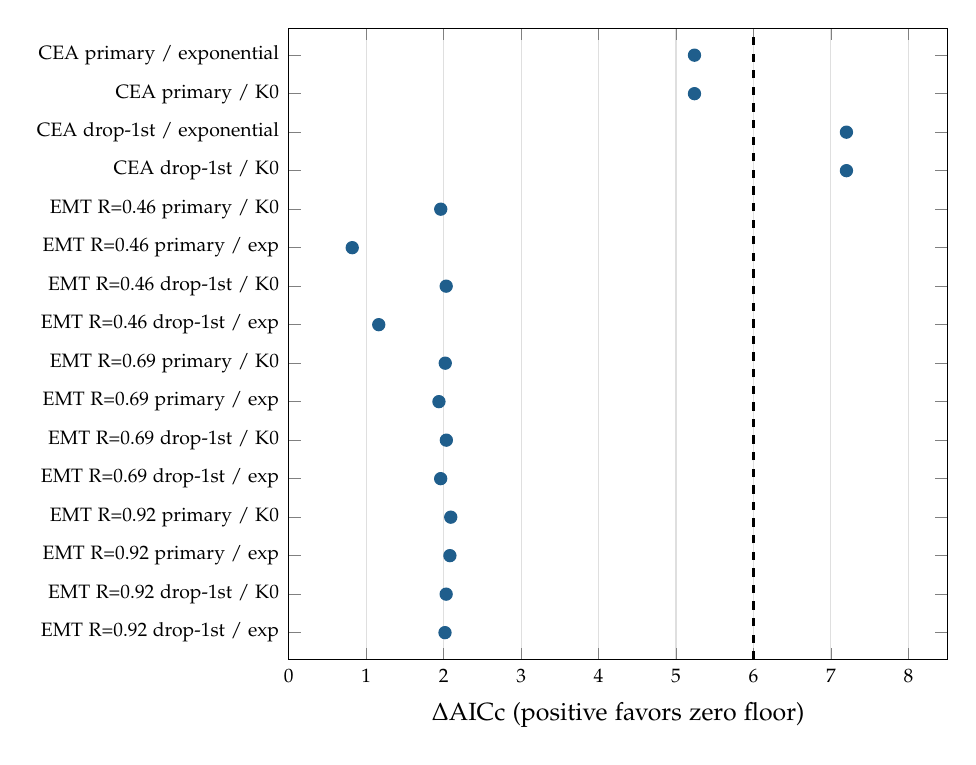
\begin{tikzpicture}
\begin{axis}[width=0.82\textwidth,height=9.6cm,xlabel={$\Delta\mathrm{AICc}$ (positive favors zero floor)},xmin=0,xmax=8.5,ymin=-0.7,ymax=15.7,ytick={0,1,2,3,4,5,6,7,8,9,10,11,12,13,14,15},yticklabels={{EMT R=0.92 drop-1st / exp},{EMT R=0.92 drop-1st / K0},{EMT R=0.92 primary / exp},{EMT R=0.92 primary / K0},{EMT R=0.69 drop-1st / exp},{EMT R=0.69 drop-1st / K0},{EMT R=0.69 primary / exp},{EMT R=0.69 primary / K0},{EMT R=0.46 drop-1st / exp},{EMT R=0.46 drop-1st / K0},{EMT R=0.46 primary / exp},{EMT R=0.46 primary / K0},{CEA drop-1st / K0},{CEA drop-1st / exponential},{CEA primary / K0},{CEA primary / exponential}},yticklabel style={font=\scriptsize},tick label style={font=\scriptsize},label style={font=\small},xmajorgrids=true,grid style={gray!25}]
\addplot[only marks,mark=*,mark size=2.2pt,accA] coordinates {(2.0170,0) (2.0322,1) (2.0805,2) (2.0915,3) (1.9613,4) (2.0344,5) (1.9389,6) (2.0203,7) (1.1619,8) (2.0324,9) (0.8194,10) (1.9623,11) (7.2000,12) (7.2000,13) (5.2381,14) (5.2381,15)};
\addplot[dashed,thick,black] coordinates {(6,-0.7)(6,15.7)};
\end{axis}
\end{tikzpicture}
\caption{Zero-floor versus positive-floor model competition ($\Delta\mathrm{AICc}>0$ favors the zero floor). Dashed line: the frozen decisive threshold $|\Delta\mathrm{AICc}|=6$. Only the CEA drop-first sensitivity crosses it; all EMT-I entries (three source separations, primary and drop-first tails, two families) lie below it, so the data neither exclude nor establish a positive floor there.}\label{fig:aicc}
\end{figure}

\subsection{Synthesis and falsification audit}
The Stage~2 synthesis is \texttt{NO-\allowbreak{}UNIVERSAL-\allowbreak{}STRUCTURAL-\allowbreak{}EXCLUSION-\allowbreak{}DETECTED}, with the structural interpretation \texttt{STRUCTURAL-\allowbreak{}VACUUM-\allowbreak{}ACCESSIBILITY-\allowbreak{}SUPPORTED}. Per criterion, \cref{tab:F} records the outcome of the preregistered failure modes.

\begin{table}[t]
\centering\small
\caption{Stage~2 falsification audit (F1--F7), as recorded in the Stage~2 synthesis.}\label{tab:F}
\begin{tabularx}{\textwidth}{@{}l>{\raggedright\arraybackslash}X>{\raggedright\arraybackslash}p{4.2cm}@{}}
\toprule
& Failure criterion & Outcome\\\midrule
F1 & Every admissible refinement path terminates before vacuum approach & Not observed\\
F2 & Common refinement produces $\Dstruct\ge\delta>0$ & Not observed (no stable positive-floor verdict)\\
F3 & Apparent approach disappears under independent representations & Not observed\\
F4 & Approach requires loss of admissibility & Not observed in the structural chambers used; not proved for all possible representations\\
F5 & Effect produced only by digitization, interpolation or window choice & Not supported (Baker downgraded; EMT needs no interpolation)\\
F6 & Continuity-like behavior only in synthetic controls & Not observed (measured lattice and published continuum profiles)\\
F7 & An independent structural chamber reproduces universal non-crossability & Not observed\\\bottomrule
\end{tabularx}
\end{table}

\paragraph{What Stage~2 has not established.} It does not prove $V\in\overline{\AYM}$. It has not delivered, with decisive precision, a single fully refinement-stable measured-data sequence $L_n\in\AYM$ with $\Dstruct(L_n,V)\to0$ under a representation-independent metric: the strongest primary CEA branch is \texttt{REFINEMENT-\allowbreak{}INDETERMINATE} and the primary EMT branch \texttt{EMT-\allowbreak{}UNCERTAINTY-\allowbreak{}LIMITED}. The absence of a detected floor is, in those branches, absence of decisive evidence for or against one; the support for accessibility comes from the convergence of branches rather than from any one decisive test.

%==============================================================
\section{Stage 3: independent spectral discreteness}\label{sec:stage3}

Stage~3 asks a different question of independent data: is there a strictly positive spectral scale for the lowest scalar excitation of pure SU(3) gauge theory? Two continuum anchors were frozen, each in its \emph{native coordinate}, and deliberately not converted into one another.

\paragraph{SPEC-I/A (Athenodorou--Teper \cite{AT20}).} The continuum $0^{++}$ ground state in units of the string tension is
\begin{equation}
\frac{M_{0^{++}}}{\sqs}=3.405(21),
\end{equation}
with the alternate extrapolation $3.391(23)$ and lower one-sigma bounds $3.384$ and $3.368$; the frozen status is \texttt{SPECTRAL-\allowbreak{}SCALE-\allowbreak{}POSITIVE}. The underlying lattice ladder (eight ensembles, $a\sqs=0.3999\to0.1038$) has $M/\sqs$ rising from $2.468(42)$ to $3.346(23)$ and positive at every level; these are lattice values, not continuum-extrapolated, and are shown only to display the approach to the continuum anchor (\cref{fig:spec}, left).

\paragraph{SPEC-I/B (Chen et al.\ \cite{Chen06}).} In the independent anisotropic-lattice study the scalar glueball mass is
\begin{equation}
r_0 M_{0^{++}}=4.16(11)(4)
\end{equation}
(statistical and anisotropy errors; conservative linear lower bound $4.01$), again \texttt{SPECTRAL-\allowbreak{}SCALE-\allowbreak{}POSITIVE}. A historical source value $4.21(11)$ was recorded as a check and \emph{not} counted as an independent Stage~3 branch.

\paragraph{Independence.} The two anchors use different actions and scale conventions ($\sqs$ versus the Sommer parameter $r_0$) and different collaborations. We do not convert between $\sqs$ and $r_0$ merely to display agreement: their independence is part of the argument, and each is positive in its own coordinate (\cref{fig:spec}, right). For context, \cref{tab:cont} lists the other continuum channels extracted from \cite{AT20}; only the $A_1^{++}$ ground state enters the verdict.

\begin{figure}[t]
\centering
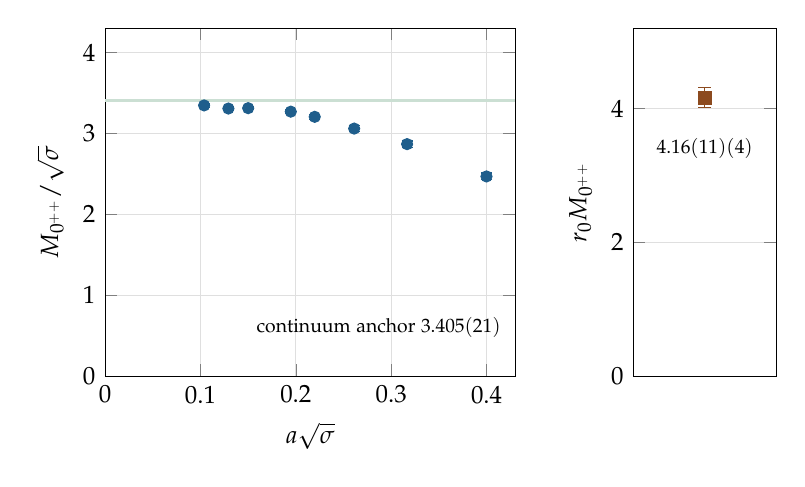
\begin{tikzpicture}
\begin{axis}[name=L,width=0.56\textwidth,height=6cm,xlabel={$a\sqrt{\sigma}$},ylabel={$M_{0^{++}}/\sqrt{\sigma}$},xmin=0,xmax=0.43,xtick={0,0.1,0.2,0.3,0.4},ymin=0,ymax=4.3,grid=major,grid style={gray!25},tick label style={font=\small},label style={font=\small}]
\fill[accC!25] (axis cs:0,3.384) rectangle (axis cs:0.43,3.426);
\addplot[only marks,mark=*,mark size=2pt,accA,error bars/.cd,y dir=both,y explicit] table[row sep=\\,x index=0,y index=1,y error index=2] {
0.39990 2.4681 0.0423\\
0.31666 2.8674 0.0384\\
0.26118 3.0596 0.0355\\
0.21982 3.2049 0.0316\\
0.19472 3.2688 0.0239\\
0.15003 3.3120 0.0204\\
0.12928 3.3075 0.0294\\
0.10383 3.3459 0.0226\\
};
\node[font=\scriptsize,anchor=south east] at (axis cs:0.425,0.35) {continuum anchor $3.405(21)$};
\end{axis}
\begin{axis}[at={(L.east)},xshift=1.5cm,anchor=west,width=0.28\textwidth,height=6cm,ylabel={$r_0M_{0^{++}}$},xmin=0,xmax=2,xtick=\empty,ymin=0,ymax=5.2,grid=major,grid style={gray!25},tick label style={font=\small},label style={font=\small}]
\addplot[only marks,mark=square*,mark size=2.4pt,accB,error bars/.cd,y dir=both,y explicit] coordinates {(1,4.16) +- (0,0.15)};
\node[font=\scriptsize,anchor=north] at (axis cs:1,3.7) {$4.16(11)(4)$};
\end{axis}
\end{tikzpicture}
\caption{Spectral positivity in native coordinates. \emph{Left:} Athenodorou--Teper lattice $M_{0^{++}}/\sqs$ against $a\sqs$ (error bars as recorded), with the continuum anchor $3.405(21)$ as a dashed line. \emph{Right:} the Chen et al.\ anchor $r_0M_{0^{++}}=4.16$ with its combined statistical-plus-anisotropy bar $(\pm0.11\pm0.04$ added linearly$)$. The panels use different coordinates and are not to be compared on one axis.}\label{fig:spec}
\end{figure}

\begin{table}[t]
\centering\small
\caption{Continuum glueball masses in units of $\sqs$ extracted from \cite{AT20} (Table~14 of the source); only the first row enters SPEC-I/A.}\label{tab:cont}
\begin{tabular}{@{}llc@{}}\toprule Channel & State & $M/\sqs$\\\midrule
$A1^{++}$ & ground & $3.405(21)$\\
$A1^{++}$ & first excitation & $5.855(41)$\\
$E^{++}$ & ground & $4.904(20)$\\
$T2^{++}$ & ground & $4.884(19)$\\
$A1^{-+}$ & ground & $5.276(45)$\\
\bottomrule\end{tabular}
\end{table}

%==============================================================
\section{BRIDGE-III: coexistence rather than identification}\label{sec:bridge}

BRIDGE-III is a deterministic evaluator over \emph{frozen statuses only}: it reads the Stage~2 status and the two SPEC-I statuses, verifies six checks, and emits an outcome; it cannot modify any earlier verdict. Its inputs and result are
\[
\begin{aligned}
&\texttt{STRUCTURAL-\allowbreak{}VACUUM-\allowbreak{}ACCESSIBILITY-\allowbreak{}SUPPORTED}\ \ (\text{Stage 2})\\
&\quad\wedge\ \texttt{SPECTRAL-\allowbreak{}SCALE-\allowbreak{}POSITIVE}\ (\text{SPEC-I/A})\ \wedge\ \texttt{SPECTRAL-\allowbreak{}SCALE-\allowbreak{}POSITIVE}\ (\text{SPEC-I/B})\\
&\quad\Longrightarrow\ \texttt{COEXISTENCE-\allowbreak{}SUPPORTED}.
\end{aligned}
\]
All six deterministic checks passed (structural status found; SPEC-I/A and SPEC-I/B statuses found; both numeric guards; theory match to pure SU(3)), and the three input files matched their recorded SHA-256 digests (\cref{app:repro}). The record explicitly states that earlier verdicts were not modified and that neither a mass-gap theorem nor a closure theorem is claimed. The project-level frozen result is \texttt{STRUCTURAL-\allowbreak{}SPECTRAL-\allowbreak{}COEXISTENCE-\allowbreak{}SUPPORTED}: within the frozen pure-SU(3) evidence architecture, structural continuity can coexist with spectral discreteness.

\begin{table}[t]
\centering\small
\caption{Margin of the frozen spectral scales above zero, each in its own native coordinate. Lower bounds are those recorded in the SPEC-I extracts (one-sigma for A; conservative linear for B).}\label{tab:margin}
\begin{tabular}{@{}llccc@{}}
\toprule
Branch & Coordinate & Central value & Lower bound & Central value $/\,\sigma$\\\midrule
SPEC-I/A & $M_{0^{++}}/\sqs$ & $3.405$ & $3.384$ & $3.405/0.021\approx162$\\
SPEC-I/B & $r_0M_{0^{++}}$ & $4.16$ & $4.01$ & $4.16/0.117\approx36$\\\bottomrule
\end{tabular}
\end{table}
(The last column divides the central value by the recorded one-sigma uncertainty, with $\sigma_B=\sqrt{0.11^2+0.04^2}\approx0.117$ used for provenance only.) Both scales are therefore many standard deviations from zero; the point of Stage~3, however, is not the size of the margin but that positivity is retained independently of the structural stage.

\subsection{Master table of frozen verdicts}\label{sec:master}
\Cref{tab:verdicts} lists every frozen verdict and stage status of both projects, with the representation tested, the question asked, and what each result rules in and out. It is the single reference against which every statement in this paper can be checked.

\begin{landscape}
{\footnotesize
\setlength{\tabcolsep}{4pt}
\begin{longtable}{@{}l>{\raggedright\arraybackslash}p{3.3cm}>{\raggedright\arraybackslash}p{3.8cm}>{\raggedright\arraybackslash}p{4.4cm}>{\raggedright\arraybackslash}p{4.6cm}>{\raggedright\arraybackslash}p{5.2cm}@{}}
\caption{Every frozen verdict and stage status of \texttt{UNNS\_YM\_GAP} (G) and \texttt{UNNS\_VACUUM\_CONTINUITY} (V). Verdict strings are quoted exactly as frozen.}\label{tab:verdicts}\\
\toprule ID & Source & Representation & Question & Verdict & Rules in / out\\\midrule\endfirsthead
\toprule ID & Source & Representation & Question & Verdict & Rules in / out\\\midrule\endhead
\bottomrule\endfoot
G1 & \texttt{UNNS\_YM\_GAP}\ YM-0 & Formalization & Frozen hypotheses, observables, null rules, refinement logic, falsification criteria & complete for the present program & In: preregistered protocol. Out: any physical claim.\\[3pt]
G2 & \texttt{UNNS\_YM\_GAP}\ YM-1 & Gauge-invariant glueball/lattice corpus & Is there a working corpus of gauge-invariant quantities? & sufficient for current work & In: data base for YM-2/3. Out: nothing physical.\\[3pt]
G3 & \texttt{UNNS\_YM\_GAP}\ YM-2A / STRUC-I & Six-node vacuum-anchored spectral ladder & Does vacuum compression (gap reduced up to $\times1024$) leave the ladder inadmissible? & vacuum-compressed branch not rejected & Out: short ladder as non-crossability evidence.\\[3pt]
G4 & \texttt{UNNS\_YM\_GAP}\ YM-2A / STRUC-PERC-I & Same ladder, four deformation families & Is fragmentation specific to approach toward the vacuum? & directionality test failed; representation/test pair falsified & Out: connectivity collapse $\equiv$ vacuum non-crossability.\\[3pt]
G5 & \texttt{UNNS\_YM\_GAP}\ YM-2B & CORR-I correlator chamber (AT20) & Does $R_{\rm contract}$ separate massive from gapless adversaries at fixed resolution? & \texttt{VACUUM-\allowbreak{}BOUNDARY DIAGNOSTIC ESTABLISHED; REFINEMENT TEST REQUIRED} (provisional) & In: fixed-resolution separation. Out: refinement stability.\\[3pt]
G6 & \texttt{UNNS\_YM\_GAP}\ YM-3A & Class C mass-anchored controls, 8 levels & Does the separation persist under common refinement? & \texttt{MODEL-\allowbreak{}REFINEMENT PERSISTENT} & In: model-family persistence. Out: measured-correlator persistence.\\[3pt]
G7 & \texttt{UNNS\_YM\_GAP}\ YM-3B & Class B Sakai--Sasaki reconstruction, 4 levels & Does the separation persist for measured data? & \texttt{DATA-\allowbreak{}INDETERMINATE} & In: central crossing at $\beta=6.71$. Out: stable falsification; stable persistence.\\[3pt]
G8 & \texttt{UNNS\_YM\_GAP}\ YM-4 & Bridge theorem under original premise & --- & not entered / cancelled & Out: any structural-to-Hamiltonian bridge.\\[3pt]
G9 & \texttt{UNNS\_YM\_GAP}\ closure & Whole project & Is a refinement-stable non-crossable vacuum boundary established? & \texttt{NOT ESTABLISHED} & Out: universal non-crossability as established; not a proof of its negation.\\[3pt]
\midrule
V0 & \texttt{UNNS\_VACUUM\_\allowbreak CONTINUITY}\ Stage 1 & Ontology $V\in\overline{\AYM\setminus\{V\}}$; VREF-I & What is meant by ``vacuum belongs to the substrate\textquotedblright{}; failure criteria F1--F7 & FROZEN (definitions; no empirical verdict) & Out: ``basin\textquotedblright{}, ``attractor\textquotedblright{}, ``fixed point\textquotedblright{}.\\[3pt]
\midrule
V1 & Baker 2022 \cite{Baker22}\ VREF-I/A & Common-refinement profiles, 3 resolutions & Is the refinement ordering interpolation-independent? & \texttt{CALIBRATION-\allowbreak{}SENSITIVE} & In: methodological warning. Out: continuity or isolation verdict.\\[3pt]
V2 & CEA 2017 \cite{Cea17}\ VREF-I/B & Connected field profile, deep tail & Zero floor vs positive floor; cross-refinement agreement & \texttt{REFINEMENT-\allowbreak{}INDETERMINATE} & In: vacuum-directed path, no floor detected. Out: absolute refinement-stable calibration; isolation.\\[3pt]
V3 & CEA 2017\ STRUC bridge & STRUC-I / STRUC-PERC-I on 5 ladders & Does refinement change regime or topology? & \texttt{ARCHITECTURE-\allowbreak{}PRESERVED} & In: structural organization stable. Out: absolute-amplitude agreement.\\[3pt]
V4 & Battelli 2019 \cite{Battelli19}\ control & Unsmoothed connected correlator, 3 ladders & Is the architecture an artifact of smearing? & \texttt{UNSMOOTHED-\allowbreak{}ARCHITECTURE-\allowbreak{}CONSISTENT} & In: corroboration. Out: independent primary distance measurement.\\[3pt]
V5 & Yanagihara 2019 \cite{Yanagihara19}\ EMT-I, $R=0.69$\,fm & Vacuum-subtracted 4-component EMT norm & Zero floor vs positive floor (decisive $|\Delta$AICc$|\ge6$) & \texttt{EMT-\allowbreak{}UNCERTAINTY-\allowbreak{}LIMITED} & In: vacuum-directed, zero floor favored numerically. Out: decisive floor exclusion; \texttt{EMT-\allowbreak{}CONTINUITY-\allowbreak{}CONSISTENT}.\\[3pt]
V6 & Yanagihara 2019\ geometry & Same at $R=0.46,\,0.92$\,fm & Is the result geometry-dependent? & \texttt{GEOMETRY-\allowbreak{}ROBUST-\allowbreak{}NO-\allowbreak{}FLOOR} & In: no floor at any tested separation. Out: floor-free proof.\\[3pt]
V7 & Stage 2 synthesis & All Stage 2 branches & Is a universal refinement-stable positive floor detected? & \texttt{NO-\allowbreak{}UNIVERSAL-\allowbreak{}STRUCTURAL-\allowbreak{}EXCLUSION-\allowbreak{}DETECTED} & Out: universal non-crossability in tested representations.\\[3pt]
V8 & Stage 2 interpretation & Same & What does V7 support? & \texttt{STRUCTURAL-\allowbreak{}VACUUM-\allowbreak{}ACCESSIBILITY-\allowbreak{}SUPPORTED} & In: accessibility (empirical). Out: $V\in\overline{\AYM}$ as a theorem.\\[3pt]
V9 & SPEC-I/A: AT20 \cite{AT20} & $M_{0^{++}}/\sqs=3.405(21)$ & Is the continuum scalar scale positive? & \texttt{SPECTRAL-\allowbreak{}SCALE-\allowbreak{}POSITIVE} & In: $\dspec>0$ in $\sqs$ units. Out: any structural statement.\\[3pt]
V10 & SPEC-I/B: Chen et al.\ \cite{Chen06} & $r_0M_{0^{++}}=4.16(11)(4)$ & Same, independent source and scale & \texttt{SPECTRAL-\allowbreak{}SCALE-\allowbreak{}POSITIVE} & In: independent positivity. Out: conversion between $\sqs$ and $r_0$.\\[3pt]
V11 & BRIDGE-III & Frozen statuses V8, V9, V10 & Do accessibility and spectral positivity coexist? & \texttt{COEXISTENCE-\allowbreak{}SUPPORTED} & In: coexistence. Out: identification; mass-gap or closure theorem.\\[3pt]
V12 & Stage 3 / project & Whole project & Project-level result & \texttt{STRUCTURAL-\allowbreak{}SPECTRAL-\allowbreak{}COEXISTENCE-\allowbreak{}SUPPORTED} & In: structural continuity can coexist with spectral discreteness (within frozen architecture). Out: Clay problem.\\[3pt]
\end{longtable}}
\end{landscape}


%==============================================================
\section{Discussion: two different notions of distance from the vacuum}\label{sec:discussion}

The central conceptual result is the separation of $\dstruct$ from $\dspec$. The program set out to test whether a positive $\dspec(E_1,E_0)=E_1-E_0$ is reflected by a positive $\dstruct$-floor. The evidence is that
\begin{equation}
\dstruct(X_n,V)\to0\ \ \text{need not imply}\ \ \dspec(E_n,E_0)\to0 .
\end{equation}
In the language of \cref{thm:sep}: the data are \emph{compatible with} a gapped, structurally accessible system, hence with a $\Delta>0$ energy functional that is discontinuous at the vacuum in the structural topology. The original program would have required the bridge condition \eqref{eq:holder}; its failure is not a failure of the gap, but of the assumption that structure controls energy.

\paragraph{Three possible readings.} By \cref{thm:sep}(d), if a genuine accessibility sequence is eventually established, at least one of the following must hold: (i) $\Pi$ is not continuous at the structural vacuum; (ii) $\mathcal E$ is not continuous at $\Omega$ in the chosen topology on $\HYM$; or (iii) the structural topology is strictly weaker, at the vacuum, than the topology induced by the excitation functional (\cref{cor:top}). We do not currently decide among them. One reason (ii) is not exotic: for an unbounded Hamiltonian, the expectation-value functional is not norm-continuous at the vacuum state in general, so the Hilbert-space half of the factorization cannot be assumed continuous without specifying the topology.

\paragraph{What the toy example shows and does not show.} \Cref{ex:corr} makes the discontinuity concrete in correlator language but is not evidence about Yang--Mills; it merely shows that accessibility and a gap are not contradictory for a natural amplitude-based metric and that the verdict depends on the metric. Whether the \uns{} structural metric behaves like the amplitude metric (accessibility at fixed gap) or like a shape metric (no accessibility) is part of what the open problem must decide.

\paragraph{Why the empirical and theorem levels are not the same claim.} The empirical coexistence is a statement about the frozen branches; the theorem is a statement about any structural--spectral system. They meet only if the Stage~2 profile windows can be embedded as a structural space $\mathcal S$ with an energy functional $\varepsilon$ and an excitation set $\Pset$, which is not currently established (\cref{rem:premise}).

%==============================================================
\section{Implications for UNNS and for the Yang--Mills interpretation}\label{sec:implications}

The mass gap should no longer be represented in \uns{} primarily as a forbidden structural region around the vacuum. The question the work leaves is deeper:
\begin{quote}
\emph{What structural mechanism allows configurations to approach the vacuum while keeping the first admissible physical excitation spectrally separated?}
\end{quote}
This redirects the program toward the structure-to-spectrum map rather than another search for a vacuum wall. Concretely, the open \uns{} theorem problem is to
\begin{enumerate}[label=(\roman*)]
\item specify the structural space $\SUNNS$ and its topology (the choice of $d$ matters, \cref{ex:corr});
\item construct $\Pi:\SUNNS\to\HYM$, the map from admissible structural configurations to Hilbert-space/spectral data of pure SU(3) Yang--Mills;
\item determine whether $\varepsilon=\mathcal E\circ\Pi$ is continuous at the structural vacuum, and if not, which factor fails (\cref{thm:sep}(d));
\item if a bridge condition of the Hölder type \eqref{eq:holder} \emph{does} hold on some sub-domain, extract the resulting exclusion radius $\delta_{\rm struct}=\min\{r,(\Delta/C)^{1/\alpha}\}$ as a testable prediction; if not, characterize the mechanism of decoupling.
\end{enumerate}
A genuinely substantial theorem would be a nontrivial statement about $\Pi$; \cref{thm:sep} only fixes what such a statement must say. In this sense the experiments did not merely flag a theorem to be proved; they identified a theorem family whose abstract member is already provable and whose difficult member is the Yang--Mills specialization.

%==============================================================
\section{Limitations and falsifiability}\label{sec:limits}

\paragraph{Not proved.} We have not proved $V\in\overline{\AYM}$ as a theorem, and we have not solved the Clay Yang--Mills problem; BRIDGE-III itself records both restrictions. We have not constructed $\Pi$, nor a representation-independent structural metric, so the premise of \cref{thm:sep}(c)--(d) is not discharged (\cref{rem:premise}).

\paragraph{Evidence limits.} (1) The Stage~2 structural states are spatial profile windows and ladders, not excitation sequences. (2) Class~B inputs are reconstructed from published figures; the YM-3B uncertainty ensemble is pointwise without covariance. (3) The primary CEA and EMT branches are indeterminate by the frozen thresholds; the Stage~2 verdict is ``supported'', not ``established''. (4) The spectral anchors are published values, not recomputed. (5) All results are for pure SU(3); no statement is made about QCD with dynamical quarks. (6) BRIDGE-III is bookkeeping over frozen statuses and adds no new inference. (7) The original picture is \texttt{NOT ESTABLISHED}, not refuted: the YM-3B crossing is statistically unresolved.

\paragraph{What would change the conclusions.} The accessibility interpretation would be weakened or falsified by: a primary branch returning a decisive positive-floor verdict ($|\Delta\mathrm{AICc}|\ge6$ against the zero floor) on adequate data; a refinement-induced regime or percolation change in STRUC-I/STRUC-PERC-I for an excitation-relevant ladder; or an instantiation of the theorem's premise in a representation-independent metric showing $\inf\Dstruct>0$ over physical excitations. Conversely, the coexistence claim would be strengthened by a decisive $\Delta\mathrm{AICc}\ge6$ at the primary EMT geometry, and by an explicit $\Pi$ for which the accessibility sequence is realized. The spectral side is falsified only by a continuum extrapolation consistent with zero for the scalar mass, which would contradict both independent anchors.

%==============================================================
\section{Conclusion: the gap is spectral, not necessarily structural}\label{sec:conclusion}

The present evidence does not support identifying the Yang--Mills mass gap with a universal structural exclusion zone around the vacuum. Instead, it supports a picture in which the vacuum remains structurally approachable while the lowest physical excitation remains spectrally separated. Mathematically, a gap implies a structural wall only under a continuity or coercivity bridge, and structural accessibility under a persisting gap forces that bridge to fail; this is elementary but pinpoints the missing assumption of the original program. The remaining task is the hard one: to build the map from \uns{} structure to Yang--Mills spectrum and to determine its topology.

%==============================================================
\appendix
\section{Supporting data tables}\label{app:data}
\subsection*{A.1 YM-3A: Class C eight-level refinement}
\begin{table}[ht]\centering\small\caption{YM-3A primary common-grid results (all matched orderings pass).}\label{tab:ym3a}
\begin{tabular}{@{}rcccc@{}}\toprule $\beta$ & $R_{\rm massive}$ & $R_{p=8}$ matched & $S_{\rm fixed}$ & $S_{\rm match}$\\\midrule
5.6924 & 0.018556 & 0.041575 & 0.708018 & 0.806712\\
5.8 & 0.012377 & 0.040156 & 1.112950 & 1.176904\\
5.8941 & 0.010214 & 0.039234 & 1.305025 & 1.345755\\
5.99 & 0.008840 & 0.038463 & 1.449513 & 1.470402\\
6.0625 & 0.008297 & 0.038108 & 1.512884 & 1.524494\\
6.235 & 0.007950 & 0.037863 & 1.555686 & 1.560841\\
6.338 & 0.007985 & 0.037888 & 1.551275 & 1.557102\\
6.5 & 0.007688 & 0.037668 & 1.589194 & 1.589194\\
\bottomrule\end{tabular}\end{table}
\subsection*{A.2 YM-3B: Class B four-level refinement}
\begin{table}[ht]\centering\small\caption{YM-3B central results and preregistered sensitivity.}\label{tab:ym3b}
\begin{tabular}{@{}rcccccc@{}}\toprule $\beta$ & $R_B$ & $R_{p=8}$ & $S_B$ & $S_B^{\rm PCHIP}$ & 95\% interval & matched order\\\midrule
6.2 & 0.088576 & 0.092825 & 0.020350 & 0.019648 & [0.004053, 0.035659] & pass\\
6.4 & 0.082775 & 0.089902 & 0.035867 & 0.036198 & [0.017167, 0.053094] & pass\\
6.71 & 0.092700 & 0.091978 & $-$0.003395 & $-$0.003948 & [$-$0.027454, 0.019320] & fail\\
6.93 & 0.082333 & 0.092774 & 0.051851 & 0.052060 & [0.024726, 0.081194] & pass\\
\bottomrule\end{tabular}\end{table}
\noindent Nested ladder lengths (L5/L6/L7) at $\beta=6.71$: $S_B=-0.007663,\,-0.006666,\,-0.003395$; at the other three $\beta$ all lengths are positive.
\subsection*{A.3 Baker calibration windows}
\begin{table}[ht]\centering\small\caption{Ratio $C=R_{23}/R_{12}$ of successive refinement distances by window and interpolation.}
\begin{tabular}{@{}ccccc@{}}\toprule window & $[u_0,u_1]$ & $C_{\rm linear}$ & $C_{\rm PCHIP}$ & class (lin/PCHIP)\\\midrule
0 & [0, 0.5] & 0.449 & 0.357 & $<$1 / $<$1\\
1 & [0.125, 0.625] & 0.546 & 0.275 & $<$1 / $<$1\\
2 & [0.25, 0.75] & 0.532 & 0.544 & $<$1 / $<$1\\
3 & [0.375, 0.875] & 0.987 & 1.036 & $<$1 / $>$1\\
4 & [0.5, 1] & 1.485 & 1.529 & $>$1 / $>$1\\
\bottomrule\end{tabular}\end{table}
\subsection*{A.4 CEA refinement mismatch}
\begin{table}[ht]\centering\small\caption{CEA energy density of the two physical refinements (R1, R2 common-linear) in the tail, $\mathrm{GeV}^2$.}
\begin{tabular}{@{}cccc@{}}\toprule $x$ (fm) & $E_{R1}$ & $E_{R2}$ & $E_{R2}/E_{R1}$\\\midrule
0.381 & 0.1242 & 0.1330 & 1.071\\
0.476 & 0.0726 & 0.0810 & 1.116\\
0.571 & 0.0409 & 0.0466 & 1.137\\
0.666 & 0.0222 & 0.0258 & 1.161\\
0.761 & 0.0117 & 0.0139 & 1.184\\
\bottomrule\end{tabular}\end{table}
\subsection*{A.5 AT20 lattice ladder}
\begin{table}[ht]\centering\small\caption{Eight AT20 ensembles: $A_1^{++}$ ground-state mass in lattice units and in $\sqs$ units.}
\begin{tabular}{@{}rccccc@{}}\toprule level & $\beta$ & lattice & $a\sqs$ & $aM$ & $M/\sqs$\\\midrule
1 & 5.6924 & $10^3\times 16$ & 0.39990 & 0.9870(90) & 2.468(42)\\
2 & 5.8 & $12^3\times 16$ & 0.31666 & 0.9080(120) & 2.867(38)\\
3 & 5.8941 & $14^3\times 16$ & 0.26118 & 0.7991(92) & 3.060(35)\\
4 & 5.99 & $18^3\times 18$ & 0.21982 & 0.7045(65) & 3.205(32)\\
5 & 6.0625 & $20^3\times 20$ & 0.19472 & 0.6365(43) & 3.269(24)\\
6 & 6.235 & $26^3\times 26$ & 0.15003 & 0.4969(29) & 3.312(20)\\
7 & 6.338 & $30^3\times 30$ & 0.12928 & 0.4276(37) & 3.308(29)\\
8 & 6.5 & $38^3\times 38$ & 0.10383 & 0.3474(22) & 3.346(23)\\
\bottomrule\end{tabular}\end{table}


\section{Reproducibility and provenance}\label{app:repro}
\noindent All structural and spectral inputs of this paper are the frozen records of the two projects; no number was re-fitted for the paper. The analytics page built from the same records verified 21 verdict strings and audited the frozen-manifest hashes below. SHA-256 digests:

\begin{tabular}{@{}>{\raggedright\arraybackslash}p{4.4cm}l@{}}\toprule Item & SHA-256\\\midrule
CORR-I v0.1.2 chamber & \texttt{\scriptsize f972c9d460cebc19ef165e66c03f971411062eba093876406ed2efe614e2deb2}\\
BRIDGE-III input \texttt{STAGE2\_STATUS.md} & \texttt{\scriptsize 991476088907af31c6d0256a992f79780e51eeef9e163d006e50ea4246e16582} \\
BRIDGE-III input \texttt{SPEC\_I\_A\_RESULT.md} & \texttt{\scriptsize 3d0d60dd827fdc953c684d8eaca0b8b9bd7d9ac14763d321a8bc39465972ba54} \\
BRIDGE-III input \texttt{SPEC\_I\_B\_RESULT.md} & \texttt{\scriptsize 0318aa14e92058facab9aa2527d1a4f34bc846400453f0f67ade0b5fd8be6caf} \\
Chen06 source PDF & \texttt{\scriptsize 66973cf81063071cf5c58d93cff86d4778b7d8f11e83eb1f3b89a21be3047f22}\\
AT20 published (SPEC-I/A) & \texttt{\scriptsize af40f084cf4f4624224af726d0bb4822e449b161b03ce38972077023cbd0ca7c}\\
AT20 arXiv v2 (SPEC-I/A) & \texttt{\scriptsize f0eb6406bf49a00d376c0be25917173426c826050046a1bf0f32987895de23d0}\\
\bottomrule\end{tabular}

\medskip
\noindent Frozen-manifest audit: 9 of 9 Stage~2 manifest entries matched their recorded digests; BRIDGE-III's three input digests matched (\cref{sec:bridge}). BRIDGE-III run timestamp (UTC): 2026-10-05T22:43:34.


%==============================================================
\begin{thebibliography}{99}\small
\bibitem{AT20} A.~Athenodorou and M.~Teper, ``The glueball spectrum of SU(3) gauge theory in 3+1 dimensions,'' JHEP \textbf{11} (2020) 172, arXiv:2007.06422.
\bibitem{Chen06} Y.~Chen \emph{et al.}, ``Glueball spectrum and matrix elements on anisotropic lattices,'' Phys.\ Rev.\ D \textbf{73} (2006) 014516, arXiv:hep-lat/0510074.
\bibitem{SS23} K.~Sakai and S.~Sasaki, ``Glueball spectroscopy in lattice QCD using gradient flow,'' Phys.\ Rev.\ D \textbf{107} (2023) 034510, arXiv:2211.15176.
\bibitem{Battelli19} N.~Battelli and C.~Bonati, ``Color flux tubes in SU(3) Yang--Mills theory: An investigation with the connected correlator,'' Phys.\ Rev.\ D \textbf{99} (2019) 114501, arXiv:1903.10463.
\bibitem{Yanagihara19} R.~Yanagihara, T.~Iritani, M.~Kitazawa, M.~Asakawa and T.~Hatsuda, ``Distribution of stress tensor around static quark--anti-quark from Yang--Mills gradient flow,'' Phys.\ Lett.\ B \textbf{789} (2019) 210--214.
\bibitem{Cea17} P.~Cea, L.~Cosmai, F.~Cuteri and A.~Papa, ``Flux tubes in the QCD vacuum,'' Phys.\ Rev.\ D \textbf{95} (2017) 114511, arXiv:1702.06437.
\bibitem{Baker22} M.~Baker, V.~Chelnokov, L.~Cosmai, F.~Cuteri and A.~Papa, ``Unveiling confinement in pure gauge SU(3): flux tubes, fields, and magnetic currents,'' arXiv:2207.08797.
\end{thebibliography}
\end{document}
